\chapter{Stato dell'arte}\label{cap:stato_arte}

Negli ultimi anni i modelli linguistici di grandi dimensioni (Large Language Model, LLM) si sono affermati come strumenti in grado di interpretare domande formulate in linguaggio naturale e di generare risposte fluenti e articolate, aprendo la strada a una nuova generazione di assistenti conversazionali. Queste capacità li rendono candidati naturali per un servizio di supporto agli studenti; tuttavia, utilizzati così come sono, i LLM presentano limiti che ne compromettono l’affidabilità proprio nei contesti in cui l’accuratezza dell’informazione è essenziale. Questo capitolo ripercorre lo stato dell’arte a partire da tali limiti, per poi presentare la Retrieval-Augmented Generation (RAG) come approccio pensato per superarli e descrivere le principali soluzioni proposte in letteratura.

\section{Limiti dei modelli linguistici in un dominio specifico}
\label{sec:problema}

Un modello linguistico di grandi dimensioni, per quanto addestrato su un corpus sterminato di testo, soffre di due limiti strutturali quando interrogato direttamente su un dominio specifico e circoscritto come quello universitario.

Il primo è la natura statica della sua conoscenza: i parametri del modello fissano ciò che esso ``sa'' al momento in cui l'addestramento si conclude, e qualunque informazione successiva a quella data come una nuova scadenza, un regolamento modificato, un importo delle tasse aggiornato, semplicemente non vi rientra. 
In \cite{zhao2023survey}, nella loro rassegna sui large language model, descrivono questo fenomeno con il termine \emph{outdatedness hallucination}: il modello genera un contenuto che era corretto al momento dell'addestramento ma non lo è più al momento dell'uso, senza alcun segnale esplicito che lo distingua da un'affermazione ancora valida, il modello stesso non ha modo di sapere che la propria conoscenza è invecchiata.

Il secondo limite riguarda l'assenza totale di accesso ai documenti specifici dell'istituzione interrogata: un LLM generico non ha mai visto i regolamenti di un ateneo, le pagine web di un singolo corso di laurea, le slide di un insegnamento particolare. Messo di fronte a una domanda che richiede questo tipo di conoscenza, non ha altra scelta che generalizzare da pattern appresi su domini affini o, più problematicamente, produrre una risposta sintatticamente corretta e sicura di sé ma priva di fondamento fattuale, un comportamento che prende il nome di \emph{hallucination}. Huang et al. \cite{huang2023survey} ne propongono una tassonomia sistematica, riconducendone le cause a limiti dei dati di addestramento (rumorosi, incompleti o distorti), a processi di allineamento che premiano risposte sicure più che corrette, e alla natura intrinsecamente stocastica del processo di
generazione del testo.

Questi due limiti si combinano in modo particolarmente dannoso nel dominio universitario, dove il costo di un errore non è astratto ma concreto e misurabile: una scadenza riportata in modo errato comporta una tassa pagata in ritardo, un requisito di ammissione frainteso comporta una domanda respinta. Kasneci et al. \cite{kasneci2023chatgpt}, discutendo opportunità e criticità dell'uso dei large language model in ambito educativo, osservano come l'assenza di garanzie sull'accuratezza fattuale sia uno degli ostacoli principali alla loro adozione diretta in contesti dove la correttezza dell'informazione fornita allo studente non è negoziabile.

La soluzione che la letteratura ha individuato per entrambi questi limiti consiste nel separare la conoscenza fattuale dal componente che genera il linguaggio: non chiedere al modello di ``ricordare'' un fatto a partire dai propri parametri, ma fornirglielo esplicitamente come contesto al momento della domanda, recuperandolo da una base documentale aggiornabile in modo indipendente dal modello stesso. È il principio alla base del Retrieval-Augmented Generation, discusso nella Sezione~\ref{sec:rag}, ed è il principio su cui si fonda l'intero sistema sviluppato in questo lavoro di tesi.

Questa non è l'unica strada percorribile: la conoscenza mancante di un LLM potrebbe, in linea di principio, essere aggiunta direttamente ai suoi parametri con un ulteriore addestramento mirato (\emph{fine-tuning}) sui documenti specifici del dominio, piuttosto che recuperata da una base esterna a ogni domanda. Ovadia et al. \cite{ovadia2024finetuning} confrontano empiricamente le due strade su compiti che richiedono conoscenza intensiva, sia per informazioni già presenti nei dati di addestramento sia per informazioni del tutto nuove, e osservano che il fine-tuning non supervisionato fatica sistematicamente ad apprendere fatti nuovi in modo affidabile --- a meno di esporre il modello a numerose riformulazioni dello stesso fatto durante l'addestramento, un costo che cresce con
ogni aggiornamento del documento sorgente --- mentre il RAG si dimostra costantemente più efficace in entrambi i casi. Per un dominio come quello universitario, dove i documenti cambiano ogni anno accademico, questo risultato ha un peso pratico diretto: un sistema a fine-tuning richiederebbe un nuovo ciclo di addestramento a ogni aggiornamento normativo, mentre un sistema RAG richiede solo di re-indicizzare il documento modificato.

Questo principio ha già trovato applicazione in sistemi conversazionali rivolti specificamente al contesto
universitario e industriale. Una presentazione più ampia di sistemi analoghi è presentata nella Sezione~\ref{sec:sistemi-simili}.

\section{Large Language Model (LLM)}\label{sec:llm}

\subsection{Che cos'è un LLM}

Un \emph{large language model} è, nella sua forma più diffusa, una rete neurale basata sull'architettura
\emph{Transformer} \cite{vaswani2017attention}, addestrata a predire il token successivo di una sequenza di testo a partire dai token che lo precedono. L'elemento che ha reso questa architettura dominante rispetto ai modelli ricorrenti che la precedevano è il meccanismo di \emph{self-attention}: ogni token della sequenza viene messo in relazione diretta con tutti gli altri, indipendentemente dalla loro distanza, e questo permette al modello di catturare dipendenze a lungo raggio nel testo senza il collo di bottiglia sequenziale delle reti ricorrenti. Soprattutto, la self-attention rende l'addestramento parallelizzabile su hardware specializzato, una condizione necessaria per scalare questi modelli alle dimensioni che oggi li caratterizzano, sia in termini di parametri sia di dati di addestramento.

% ---------------------------------------------------------------------------
% Tokenizzazione
% ---------------------------------------------------------------------------
Prima di poter essere elaborato da un LLM, il testo deve essere convertito in una sequenza di unità discrete, i \emph{token}. Un token non coincide necessariamente con una parola: le parole più frequenti corrispondono in genere a un singolo token, mentre quelle meno comuni vengono spezzate in più frammenti sub-lessicali, fino ad arrivare, nei casi limite, ai singoli caratteri. La segmentazione è stabilita da un \emph{tokenizer}, un algoritmo che apprende da un corpus di riferimento quali frammenti di testo ricorrono più spesso. Il più diffuso, il \emph{Byte-Pair Encoding} (BPE), parte dai singoli caratteri e fonde iterativamente le coppie di simboli adiacenti più frequenti, fino a costruire un vocabolario di dimensione prefissata, tipicamente dell'ordine di decine o centinaia di migliaia di token. Come illustra la Figura~\ref{fig:tokenizzazione}, a ogni token del vocabolario è associato un identificativo numerico, ed è questa sequenza di numeri, e non il testo, che il modello riceve in ingresso e produce in uscita. In questo modo un vocabolario finito è sufficiente a rappresentare qualunque testo, comprese parole mai incontrate durante l'addestramento.

La tokenizzazione ha una conseguenza pratica diretta: tutte le grandezze che caratterizzano un LLM sono misurate in token, non in parole o in caratteri. In particolare, la \emph{finestra di contesto}, ovvero il numero massimo di token che il modello può elaborare in un'unica interazione, prompt e risposta compresi, va da poche migliaia a centinaia di migliaia di token a seconda del modello, e pone un limite diretto alla quantità di testo recuperato (Sezione~\ref{sec:rag}) che può essere fornita come contesto per una singola domanda. Il numero di token necessari a rappresentare uno stesso contenuto, inoltre, varia da una lingua all'altra: Petrov et al. \cite{petrov2023unfairness} mostrano che i tokenizer, addestrati su corpus in cui l'inglese è prevalente, segmentano in genere le altre lingue in un numero maggiore di token. A parità di contenuto, quindi, un documento in italiano può occupare una porzione della finestra di contesto più ampia del suo equivalente in inglese.

\begin{figure}[H]
  \centering
  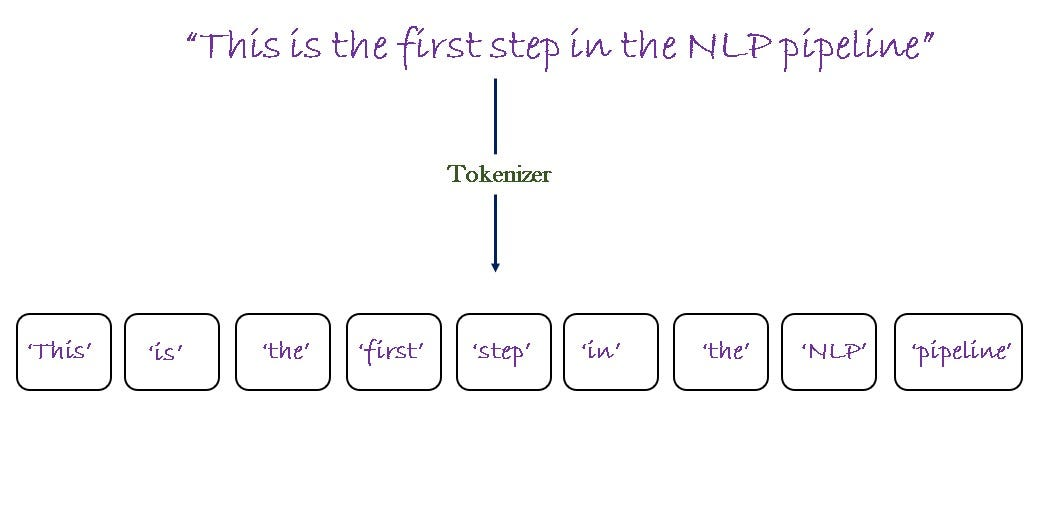
\includegraphics[width=0.99\textwidth]{assets/tokenizer.jpg}
  \caption{Tokenizzazione di una domanda in linguaggio naturale. Il tokenizer segmenta il testo in token. A ciascun token è associato un
    identificativo intero $i_k$ nel vocabolario del modello. La segmentazione mostrata è a scopo illustrativo:
    quella effettiva dipende dal tokenizer del modello considerato.}
  \label{fig:tokenizzazione}
\end{figure}

% ---------------------------------------------------------------------------
% Generazione auto-regressiva
% ---------------------------------------------------------------------------
In fase di generazione, i LLM operano in modo \emph{auto-regressivo}. Data una sequenza di token $x_1, \dots, x_t$, il modello calcola una distribuzione di probabilità sull'intero vocabolario per il token successivo, $P(x_{t+1} \mid x_1, \dots, x_t)$; da questa distribuzione viene scelto un token, il più probabile oppure uno campionato secondo la strategia di \emph{decoding} adottata, che viene accodato alla sequenza e diventa a sua volta parte del contesto per il passo seguente. Il procedimento si ripete un token alla volta, finché il modello non produce un token speciale di fine sequenza o non raggiunge un limite di lunghezza prefissato. La probabilità di un'intera sequenza si scompone quindi nel prodotto delle probabilità di ciascun token, condizionate ai token che lo precedono:
\begin{equation}
  P(x_1, \dots, x_T) = \prod_{t=1}^{T} P(x_t \mid x_1, \dots, x_{t-1}).
  \label{eq:autoregressivo}
\end{equation}
Nell'architettura Transformer questo vincolo è imposto da una \emph{maschera causale} applicata alla self-attention, che impedisce a ciascun token di considerare quelli che lo seguono. Per questo motivo i LLM generativi adottano in genere la variante \emph{decoder-only} dell'architettura, a differenza di modelli come BERT, che osservano l'intera sequenza in entrambe le direzioni e non sono pensati per generare testo. La maschera causale spiega anche perché addestramento e generazione abbiano costi così diversi: in addestramento, la sequenza è nota per intero e il modello può calcolare in parallelo le previsioni per tutte le posizioni; in generazione, invece, ogni token dipende da quelli prodotti in precedenza, e il processo è intrinsecamente sequenziale. Ne derivano due conseguenze rilevanti per questo lavoro. La prima riguarda i tempi di risposta, che crescono con la lunghezza del testo generato oltre che con quella del contesto fornito. La seconda riguarda l'affidabilità: il modello non produce la risposta nel suo insieme né rivede quanto ha già scritto, ma sceglie a ogni passo una continuazione plausibile del testo; un token errato entra nel contesto e condiziona tutti i successivi, e il campionamento introduce la componente stocastica richiamata nella Sezione~\ref{sec:problema}.

% ---------------------------------------------------------------------------
% Le tre fasi dell'addestramento
% ---------------------------------------------------------------------------
L'addestramento di un LLM avviene tipicamente in tre fasi successive, illustrate nella Figura~\ref{fig:llm-training}. Nella prima, il \emph{pre-training}, il modello
viene esposto a un corpus testuale di dimensioni enormi --- miliardi o migliaia di miliardi di token raccolti dal web, da libri, da codice sorgente --- con il solo obiettivo di predire il token successivo. Questa fase, auto-supervisionata e quindi priva di etichette fornite da esseri umani, fa emergere la competenza linguistica e una parte significativa della conoscenza fattuale del modello, codificata implicitamente nei suoi parametri \cite{zhao2023survey}.
Un modello che ha completato solo questa fase, tuttavia, non è ancora un assistente conversazionale: è un sistema di completamento testuale, che tende a proseguire il prompt ricevuto piuttosto che a rispondere a una domanda. La seconda fase, l'\emph{instruction-tuning}, affina il modello pre-addestrato in modo supervisionato su coppie istruzione-risposta scritte da esseri umani, insegnandogli a seguire le istruzioni ricevute e a rispondere nella forma attesa.

La terza fase, l'\emph{allineamento}, adatta ulteriormente il comportamento del modello alle preferenze umane, tipicamente tramite \emph{reinforcement learning from human feedback} (RLHF). Come mostra la parte inferiore della Figura~\ref{fig:llm-training}, questa fase si articola in due passaggi: prima si addestra un modello di ricompensa (\emph{reward model}) su confronti tra risposte alternative, ordinate per qualità da annotatori umani; poi si aggiorna iterativamente il modello linguistico con tecniche di apprendimento per rinforzo, usando come segnale la ricompensa stimata da quel modello. Ouyang et al. \cite{ouyang2022instructgpt}, nel lavoro che ha introdotto InstructGPT, mostrano che le ultime due fasi contano non meno della scala del modello nel renderlo utile e sicuro dal punto di vista comportamentale: un modello InstructGPT da 1,3 miliardi di parametri, sottoposto a instruction-tuning e RLHF, viene preferito dai valutatori umani a un modello GPT-3 da 175 miliardi di parametri privo di questo affinamento.

Sono quindi la seconda e la terza fase a rendere un LLM capace di rispondere in modo pertinente nella forma a una domanda posta in linguaggio naturale. Il modello resta però, come discusso nella Sezione~\ref{sec:problema}, incapace di garantire che il contenuto della risposta sia corretto o aggiornato. Né l'instruction-tuning né l'allineamento affrontano questo limite, perché esso riguarda la conoscenza codificata nei parametri e non il comportamento del modello: la conoscenza fattuale si forma quasi interamente nel pre-training, mentre le fasi successive modificano il comportamento del modello senza aggiungere, se non marginalmente, nuova conoscenza.

\begin{figure}[H]
  \centering
  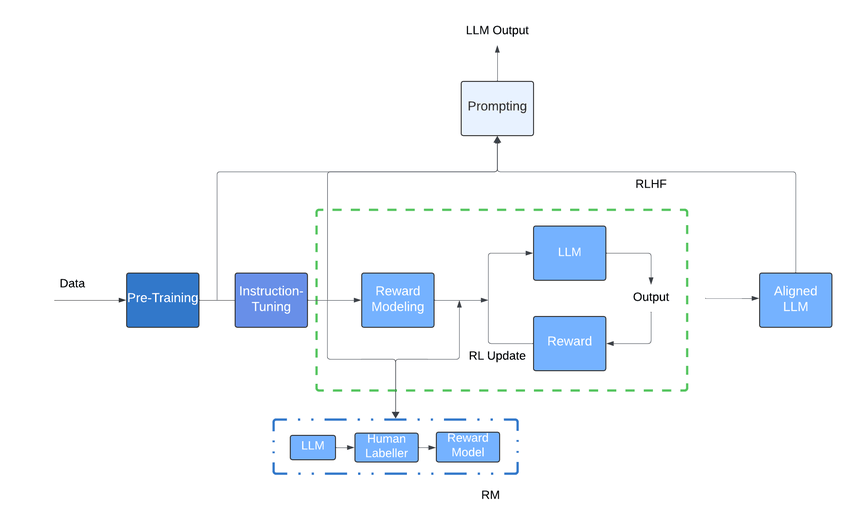
\includegraphics[width=0.9\textwidth]{assets/A-basic-flow-diagram-depicting-various-stages-of-LLMs-from-pre-training-to.png}
  \caption{Le fasi che portano dai dati grezzi a un LLM allineato e utilizzabile tramite prompting: pre-training,
    instruction-tuning e, infine, l'allineamento tramite \emph{reward modeling} (RM, in basso: un modello di
    ricompensa addestrato su confronti prodotti da annotatori umani) e \emph{reinforcement learning from human
    feedback} (RLHF, al centro: un ciclo iterativo che aggiorna l'LLM in base al segnale del modello di ricompensa).}
  \label{fig:llm-training}
\end{figure}

% ---------------------------------------------------------------------------
% Leggi di scala
% ---------------------------------------------------------------------------
Un altro aspetto, rilevante per la scelta dei modelli discussa nella sezione seguente, è il legame tra le dimensioni di un modello e la qualità delle sue previsioni. Kaplan et al. \cite{kaplan2020scaling} hanno misurato sperimentalmente come varia l'errore di predizione di un modello linguistico, cioè quanto spesso e quanto nettamente il modello sbaglia nel prevedere il token successivo, al variare di tre fattori: il numero di parametri del modello, la quantità di dati usati per addestrarlo e la potenza di calcolo complessivamente impiegata. Il risultato è una relazione sorprendentemente regolare, detta \emph{legge di scala} (\emph{scaling law}): finché gli altri due fattori non fanno da collo di bottiglia, l'errore diminuisce secondo una legge di potenza al crescere di ciascun fattore. In termini intuitivi, moltiplicare un fattore per una stessa quantità produce sempre lo stesso miglioramento in termini relativi. Secondo le stime degli autori, per esempio, raddoppiare il numero di parametri riduce l'errore di circa il 5\%, sia che si passi da 10 a 20 milioni di parametri, sia che si passi da 500 milioni a un miliardo. La Figura~\ref{fig:scaling} mostra questo andamento: su assi in scala logaritmica, le tre relazioni appaiono come rette discendenti.

Ne derivano due conseguenze. La prima è che un modello più grande, a parità di architettura e di dati di addestramento, è in genere più capace: è questa relazione, osservata ancor prima della diffusione dei moderni LLM conversazionali, a motivare l'esistenza di famiglie di modelli disponibili in più taglie, come Qwen2.5-7B e Qwen2.5-14B discussi nella sezione seguente. La seconda è che ogni ulteriore miglioramento costa sempre di più in termini assoluti: per ridurre l'errore di un'altra frazione fissa occorre ogni volta moltiplicare le risorse, e il modello più grande richiede più memoria e più tempo di calcolo per ogni risposta generata e per il training. La scelta della taglia è quindi un compromesso tra qualità delle risposte e risorse disponibili.

\begin{figure}[H]
  \centering
  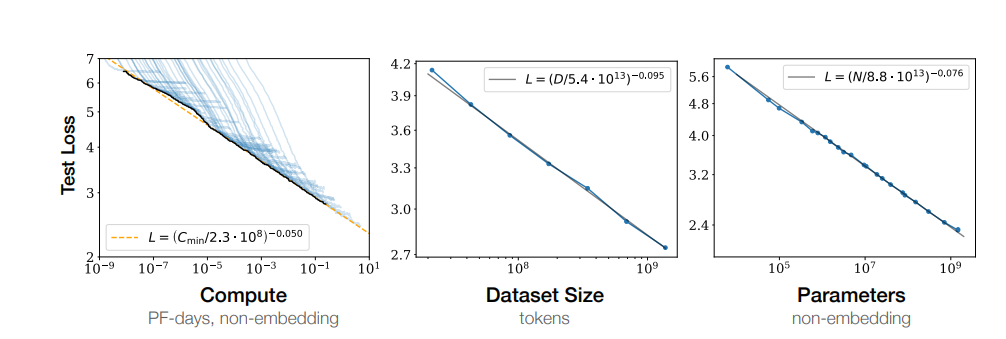
\includegraphics[width=0.9\textwidth]{assets/scale_law.png}
  \caption{Le prestazioni del modello linguistico migliorano in modo continuo man mano che aumentiamo la dimensione del modello, la dimensione del dataset e la quantità di calcolo usata per l'addestramento. Per ottenere prestazioni ottimali, tutti e tre i fattori devono essere aumentati insieme. Fonte: Kaplan et al. \cite{kaplan2020scaling}}
  \label{fig:scaling}
\end{figure}


% ---------------------------------------------------------------------------
% In-context learning
% ---------------------------------------------------------------------------
Al crescere della scala emerge anche una capacità che non corrisponde a una specifica fase di addestramento, ma che è rilevante per inquadrare il
funzionamento di un sistema RAG come quello di questo lavoro: l'\emph{in-context learning}. Brown et al.
\cite{brown2020gpt3}, presentando GPT-3, osservano che un modello linguistico sufficientemente grande può adattare il proprio comportamento a un compito nuovo semplicemente a partire da istruzioni o esempi forniti nel testo del prompt, senza alcun aggiornamento dei suoi parametri. È precisamente questo meccanismo, e non un nuovo addestramento, che un sistema RAG sfrutta quando fornisce al modello un contesto recuperato al momento della domanda (Sezione~\ref{sec:rag}): il modello non apprende un fatto nuovo in modo permanente, ma lo usa temporaneamente, limitatamente alla singola interazione in cui compare nel prompt.

% ---------------------------------------------------------------------------
% Closed-weight vs open-weight
% ---------------------------------------------------------------------------
Ai fini di questo lavoro è rilevante, infine, la distinzione tra modelli \emph{closed-weight}, accessibili solo tramite
un'interfaccia remota gestita dal fornitore e generalmente a pagamento, e modelli \emph{open-weight}, i cui parametri sono
pubblicati e possono essere eseguiti su hardware proprio. La scelta di adottare esclusivamente modelli open-weight risponde a due esigenze. La prima è il contenimento dei costi: i servizi closed-weight sono tipicamente tariffati in base al numero di token elaborati, per cui la spesa cresce con il numero di domande ricevute ed è difficile da prevedere per un servizio rivolto a un'intera università; un modello eseguito in locale comporta invece un costo legato essenzialmente all'hardware e al suo funzionamento, indipendente dal volume di utilizzo. La seconda è la tutela delle informazioni dell'ateneo: con un modello closed-weight, a ogni interrogazione la domanda dello studente e i documenti recuperati per rispondere verrebbero inviati a un fornitore esterno, mentre l'esecuzione in locale permette di non affidare a terzi documenti, contenuti del sito e informazioni proprietarie. Per questi motivi, tutti i modelli generativi considerati in
questo lavoro, descritti nella sezione seguente, sono modelli open-weight eseguibili interamente in locale.

\subsection{LLM valutati}

Il sistema sviluppato in questo lavoro è stato valutato con quattro LLM open-weight, scelti tra
quelli eseguibili sull'hardware a disposizione. Per tre di essi questo è possibile solo ricorrendo a una
quantizzazione. La \emph{quantizzazione} riduce la precisione numerica con cui sono memorizzati i pesi di un modello,
per esempio da 16 a 4 bit per peso: la memoria occupata si riduce di circa quattro volte, al prezzo di una possibile
perdita di qualità delle risposte. I tre modelli quantizzati sono serviti nella variante \emph{AWQ}
(\emph{Activation-aware Weight Quantization}), uno
schema di quantizzazione post-addestramento a 4 bit proposto da Lin et al.\ \cite{lin2024awq}. Gli autori osservano
che una piccola frazione dei pesi di un modello, quelli associati ai canali di attivazione di ampiezza maggiore,
contribuisce in modo sproporzionato all'errore di quantizzazione. AWQ individua questi pesi salienti a partire dalle
statistiche di attivazione, anziché dalla sola magnitudine dei pesi, e li protegge applicando un fattore di scala
per canale prima della quantizzazione: in questo modo la perdita di qualità si riduce drasticamente rispetto a uno
schema uniforme, senza richiedere un nuovo addestramento né una fase di backpropagation. Il quarto modello,
Llama-3.1-8B, è invece eseguito nella versione originale non quantizzata, con pesi in formato BF16 (numeri a 16 bit, la precisione con cui il modello è distribuito).

I quattro modelli confrontati sono:

\begin{itemize}
  \item \textbf{Qwen2.5-14B-Instruct-AWQ} e \textbf{Qwen2.5-7B-Instruct-AWQ}, due taglie della famiglia Qwen2.5
    sviluppata da Alibaba Cloud \cite{qwen2024technical}, che differiscono di un fattore 2 nel numero di parametri
    (14 contro 7 miliardi). Gli autori riportano un corpus di pre-training di 18 mila miliardi di token, più del
    doppio dei 7 mila miliardi della generazione precedente (Qwen2), con particolare attenzione a codice e
    matematica, e un supporto multilingue esteso a oltre 29 lingue, italiano compreso. Entrambe le varianti posseggono una finestra di contesto
    di 128k token;
  \item \textbf{Mistral-Nemo-12B-AWQ}, sviluppato congiuntamente da Mistral AI e NVIDIA
    \cite{mistralai2024nemo}, un modello da 12 miliardi di parametri con una finestra di contesto di 128k token.
    Introduce un nuovo tokenizer, Tekken, che secondo gli autori rappresenta il testo con circa il 30\% di token in
    meno rispetto al tokenizer dei precedenti modelli Mistral su codice sorgente e su diverse lingue europee, tra
    cui l'italiano, e risulta più efficiente del tokenizer di Llama~3 per circa l'85\% delle lingue. Il modello è
    stato inoltre addestrato con \emph{quantization awareness}, una procedura pensata per consentire l'inferenza in
    FP8, cioè con pesi a 8 bit;
  \item \textbf{Meta-Llama-3.1-8B-Instruct}, appartenente alla famiglia Llama~3 di Meta \cite{grattafiori2024llama3},
    composta da tre taglie dense (8, 70 e 405 miliardi di parametri) addestrate su oltre 15 mila miliardi di token,
    con una finestra di contesto di 128k token. Gli autori dichiarano un supporto ufficiale per otto lingue,
    italiano compreso, e un addestramento specifico per l'uso di strumenti esterni (\emph{tool calling}), una
    capacità agentica non rilevante per l'uso puramente conversazionale che ne fa questo sistema.
\end{itemize}

Tutti e quattro i modelli condividono la stessa architettura di fondo, il Transformer decoder-only auto-regressivo, e differiscono principalmente per numero di parametri, dati e
procedura di addestramento e tokenizer, oltre che per il formato dei pesi: Llama-3.1-8B è l'unico eseguito senza
quantizzazione, e di questa differenza occorre tenere conto nell'interpretare il confronto, perché una parte del
divario di qualità o di latenza rispetto agli altri modelli può dipendere dal formato più che dal modello in sé.
La Tabella~\ref{tab:llm_comparison} ne riassume le caratteristiche principali, mentre il confronto sistematico in termini di qualità della risposta generata, latenza e comportamento sulle diverse
categorie del dataset di test è presentato nel Capitolo~\ref{cap:validazione}.

\begin{table}[H]
    \centering
    \footnotesize
    \setlength{\tabcolsep}{4pt}
    \renewcommand{\arraystretch}{1.35}
    \begin{tabularx}{\textwidth}{@{} L{3.4cm} C{1.2cm} C{1.6cm} C{1.4cm} C{1.4cm} >{\raggedright\arraybackslash}X @{}}
        \toprule
        \textbf{Modello} & \textbf{Param.} & \textbf{Contesto} & \textbf{Formato} & \textbf{VRAM (pesi)} & \textbf{Caratteristiche principali} \\
        \midrule
        \textbf{Qwen2.5-14B-Instruct-AWQ}
            & 14,7 mld
            & 128k
            & AWQ 4 bit
            & $\sim$9--10 GB
            & Pre-training su 18 mila miliardi di token; oltre 29 lingue, italiano compreso. \\
        \midrule
        \textbf{Qwen2.5-7B-Instruct-AWQ}
            & 7,6 mld
            & 128k
            & AWQ 4 bit
            & $\sim$5--6 GB
            & Stessa famiglia del 14B con circa metà dei parametri: minore latenza e occupazione di memoria. \\
        \midrule
        \textbf{Mistral-Nemo-12B-AWQ}
            & 12,2 mld
            & 128k
            & AWQ 4 bit
            & $\sim$8--9 GB
            & Tokenizer Tekken, più compatto sull'italiano rispetto ai precedenti tokenizer Mistral. \\
        \midrule
        \textbf{Meta-Llama-3.1-8B-Instruct}
            & 8,0 mld
            & 128k
            & BF16 \newline
            & $\sim$16 GB
            & Pre-training su oltre 15 mila miliardi di token; otto lingue supportate, italiano compreso. \\
        \bottomrule
    \end{tabularx}
    \caption{Caratteristiche dei quattro modelli generativi valutati.}
    \label{tab:llm_comparison}
\end{table}


\section{RAG (Retrieval-Augmented Generation)} \label{sec:rag}

Il \emph{Retrieval-Augmented Generation} è il paradigma che Lewis et al. \cite{lewis2020retrieval} propongono per superare i due limiti discussi nella Sezione~\ref{sec:problema}: invece di affidarsi esclusivamente alla conoscenza codificata nei parametri del modello, il sistema recupera prima, da una base documentale esterna e aggiornabile, i frammenti (in inglese \emph{chunk}) di testo più pertinenti alla domanda ricevuta, e li fornisce al modello linguistico come contesto su cui basare la risposta. Il principio di fondo è separare nettamente \emph{cosa il sistema sa}, cioè l'insieme dei documenti indicizzati, che può essere aggiornato in qualunque momento senza bisogno di un nuovo addestramento, da \emph{come il sistema si esprime}, compito che resta demandato interamente al modello linguistico. Gao et al. \cite{gao2023ragsurvey}, nella loro rassegna sul tema, inquadrano questo principio come la risposta più diretta proprio ai limiti di conoscenza statica e di verificabilità discussi in precedenza: un'affermazione generata dal modello può essere ricondotta a un frammento di testo specifico, citabile e verificabile, invece che
derivare implicitamente e in modo opaco dai suoi parametri. La figura \ref{fig:rag-pipeline} mostra quella che è una pipeline generica di un sistema RAG.

\begin{figure}[H]
  \centering
  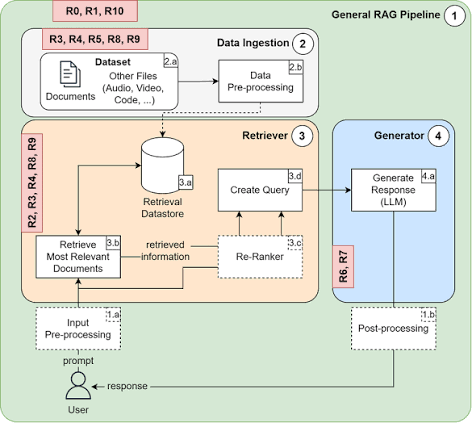
\includegraphics[width=0.6\textwidth]{assets/rag_pipeline.png}
  \caption{Schema generale di una pipeline RAG (1). Nella fase di \emph{data ingestion} (2), i documenti
  e gli altri file della collezione (2.a) vengono pre-elaborati (2.b) e indicizzati in un archivio per il
  recupero (3.a). Al momento della domanda, il prompt dell'utente viene eventualmente pre-elaborato (1.a) e
  passato al \emph{retriever} (3), che recupera i documenti più pertinenti (3.b), li riordina facoltativamente
  tramite un \emph{re-ranker} (3.c) e costruisce la richiesta da inviare al modello (3.d). Il
  \emph{generator} (4) produce la risposta tramite un LLM (4.a), che può essere post-elaborata (1.b) prima di
  essere restituita all'utente. I riquadri tratteggiati indicano componenti opzionali.}
  \label{fig:rag-pipeline}
\end{figure}

\subsection{Embedding e ricerca per similarità}\label{subsec:embedding}

Il primo problema che un sistema RAG deve risolvere è, dato un testo, come rappresentarlo in una forma che permetta
di confrontarne il significato con quello di una domanda. La soluzione standard è l'\emph{embedding}: una rete neurale
proietta ogni porzione di testo (un documento, o più spesso un suo frammento) in un vettore di numeri reali di
dimensione fissa, costruito in modo che frammenti dal significato simile vengano proiettati in punti vicini dello
spazio vettoriale. La vicinanza tra due vettori $\mathbf{u}$ e $\mathbf{v}$ si misura tipicamente con la
\emph{similarità coseno}, ovvero il coseno dell'angolo compreso tra i due vettori:
\begin{equation}
  \cos(\mathbf{u}, \mathbf{v}) = \frac{\mathbf{u} \cdot \mathbf{v}}{\lVert \mathbf{u} \rVert \, \lVert \mathbf{v} \rVert},
  \label{eq:coseno}
\end{equation}
che vale 1 per vettori con la stessa direzione e diminuisce man mano che le loro direzioni divergono.

Il punto di partenza per costruire modelli di embedding è in genere Bidirectional Encoder Representations
from Transformers (\emph{BERT}), proposto da Devlin et al.\ \cite{devlin2019bert}. A differenza dei LLM generativi descritti in precedenza, BERT utilizza solo la parte \emph{encoder} del Transformer: ogni token osserva
l'intera sequenza in entrambe le direzioni, e il modello produce per ciascun token un vettore che ne rappresenta il
significato nel contesto, senza generare testo. BERT viene pre-addestrato su grandi quantità di testo a ricostruire
parole mascherate casualmente all'interno delle frasi, e poi specializzato tramite \emph{fine-tuning} su compiti di
comprensione del linguaggio: la classificazione di un testo (per esempio l'analisi del sentiment), il riconoscimento
di entità nominate come persone e luoghi, l'individuazione della risposta a una domanda all'interno di un passaggio
dato, e la classificazione di coppie di frasi, per esempio per stabilire se due frasi sono parafrasi l'una dell'altra.

Nessuno di questi compiti, tuttavia, richiede di produrre un singolo vettore che rappresenti un'intera frase, e BERT
non è addestrato a farlo. Per confrontare due testi, BERT li riceve concatenati in un'unica sequenza e restituisce un
punteggio per la coppia, secondo un'architettura detta \emph{cross-encoder}. Reimers e Gurevych \cite{reimers2019sbert}
osservano che questo approccio è impraticabile per il recupero: ogni coppia richiede un passaggio completo attraverso
la rete, e trovare la coppia più simile in una collezione di 10.000 frasi richiede circa 50 milioni di passaggi, pari a
circa 65 ore di calcolo. D'altra parte, ricavare un vettore per ciascuna frase da BERT così com'è, per esempio facendo
la media dei vettori dei suoi token, produce embedding di bassa qualità.

La loro soluzione, Sentence-BERT (SBERT), affina BERT proprio per produrre embedding di frase confrontabili tramite la
similarità coseno. Durante l'addestramento, i due testi di ogni coppia non vengono concatenati, ma attraversano
separatamente la stessa rete, con gli stessi pesi; i due vettori risultanti vengono confrontati, e l'errore commesso
nel valutare la relazione tra i due testi (per esempio, se si tratta di parafrasi) viene usato per aggiornare i pesi.
Questa configurazione è detta \emph{siamese}, perché equivale a due copie gemelle della stessa rete. La condivisione dei
pesi garantisce che entrambi i testi vengano trasformati dalla stessa funzione, e quindi proiettati nello stesso
spazio, mentre l'addestramento fa sì che in questo spazio la similarità coseno rifletta la somiglianza di significato.
Una volta addestrata, la rete può calcolare l'embedding di ogni frammento una sola volta e indipendentemente dagli altri,
e il confronto con una domanda si riduce a una similarità coseno tra vettori già pronti: il tempo necessario a trovare
la coppia più simile tra 10.000 frasi scende così da circa 65 ore a circa 5 secondi.

Sentence-BERT è pensato per misurare la somiglianza tra frasi; nel recupero, invece, occorre confrontare una domanda
breve con passaggi di testo più lunghi che ne contengono la risposta. Karpukhin et al.\ \cite{karpukhin2020dpr}
applicano lo stesso principio a questo compito con il \emph{Dense Passage Retriever} (DPR), composto da due encoder
basati su BERT, uno per le domande e uno per i passaggi, addestrati su coppie domanda-passaggio in modo che l'embedding
di una domanda risulti vicino a quello del passaggio che contiene la risposta. Gli autori mostrano come DPR superi nettamente i metodi lessicali classici come BM25, che assegna un punteggio a ciascun documento in base alle parole che ha in
comune con la domanda, pesate secondo la loro frequenza nel documento e la loro rarità nella collezione.

Il vantaggio deriva dal fatto che un retriever basato su embedding confronta significati e non parole: una domanda come
``quando si paga la seconda rata?'' può essere associata a un passaggio che parla di ``scadenza del secondo versamento'',
pur avendo con esso quasi nessuna parola in comune. Per questo i retriever basati su embedding vengono detti
\emph{densi}, in contrapposizione alle rappresentazioni \emph{sparse} dei metodi lessicali come BM25, che descrivono un
testo con un vettore grande quanto l'intero vocabolario e composto quasi interamente da zeri. I metodi lessicali
restano comunque competitivi quando conta la corrispondenza esatta di un termine, come nel caso di codici o nomi propri.

Una domanda e un documento vengono quindi confrontati non piu sulla
base delle parole esatte che condividono, ma sulla distanza tra i rispettivi vettori nello spazio
degli embedding, calcolato in modo efficiente anche su milioni di candidati tramite strutture
dati specializzate (indici vettoriali) mantenute da un database vettoriale dedicato.

Un confronto esaustivo di un vettore query con ogni singolo vettore indicizzato (ricerca
esatta) diventa proibitivo già a poche centinaia di migliaia di frammenti, ben al di sotto della  scala di molti corpora documentali reali. I database vettoriali si affidano a una ricerca approssimata del vicino piu prossimo, che rinuncia alla garanzia di trovare sempre il risultato esatto in cambio di un tempo di
ricerca molto piu basso. Malkov e Yashunin \cite{malkov2018hnsw} propongono uno degli schemi più diffusi a
questo scopo, Hierarchical Navigable Small World (HNSW): un grafo multilivello in cui ogni
nodo rappresenta un vettore indicizzato, organizzato in strati via via piu densi, in cui la ricerca parte dallo strato piu rado (pochi nodi, collegamenti a lungo raggio) e scende progressivamente verso strati piu fitti, restringendo il raggio di ricerca a ogni passo; un meccanismo che ottiene un tempo di ricerca che cresce in modo logaritmico con il numero $N$ di vettori
indicizzati, $O(\log N)$, invece che linearmente, $O(N)$, come nella ricerca esatta.

\subsection{Ricerca ibrida e fusione dei risultati}

La ricerca per sola similarità vettoriale (\emph{dense retrieval}), tuttavia, ha un punto debole noto: tende a
performare peggio dei metodi lessicali classici (in particolare \emph{BM25} \cite{robertson2009bm25}) proprio sui termini rari o molto specifici: un codice di corso, una sigla normativa, un nome
proprio, che un embedding generico fatica a distinguere ma che un confronto esatto di parole individua senza
ambiguità. La letteratura piu recente raccomanda perciò l'adozione della \emph{ricerca ibrida} (\emph{hybrid search}): eseguire in parallelo una ricerca densa e una ricerca lessicale sparsa,
e fonderne i risultati in un'unica classifica. Una delle tecniche di fusione più diffuse a questo scopo,  è la \emph{Reciprocal Rank Fusion} (RRF), proposta da Cormack et al. \cite{cormack2009rrf}: per ogni documento si guarda non il punteggio ottenuto nelle due ricerche, ma solo la sua \emph{posizione} in ciascuna classifica e si sommano gli inversi di queste posizioni per ottenere un punteggio finale. Un documento che compare ai primi posti in entrambe le classifiche ottiene così un punteggio alto, uno che compare in alto in una sola delle due un punteggio intermedio. Il vantaggio pratico di questo meccanismo è che permette di fondere le due classifiche senza dover rendere confrontabili i punteggi originali delle due ricerche, cosa altrimenti problematica, perché il punteggio di una ricerca densa e quello di una ricerca lessicale sono calcolati in modo diverso e non sono direttamente comparabili tra loro.
\subsection{Reranking}

Il risultato della ricerca ibrida è però, tipicamente, solo una prima scrematura. Per restare efficienti su un
indice di grandi dimensioni, entrambe le sue componenti valutano ciascun frammento senza che un modello lo legga
mai insieme alla domanda. BM25 si limita a contare le parole in comune; nella componente densa, l'embedding di
ciascun frammento viene calcolato una volta per tutte, in fase di indicizzazione e quindi prima ancora di conoscere
la domanda, e al momento della ricerca viene soltanto confrontato con l'embedding della domanda tramite la
similarità coseno (Sottosezione~\ref{subsec:embedding}). Il vettore di un frammento deve perciò riassumerne l'intero
contenuto senza sapere quale aspetto interesserà a chi interroga il sistema: un frammento sulle tasse universitarie
è rappresentato sempre dallo stesso vettore, sia che la domanda riguardi la scadenza della seconda rata, sia che
riguardi l'importo previsto per una specifica fascia di reddito. Questa compressione comporta inevitabilmente una
perdita di dettaglio, e un frammento solo genericamente pertinente può finire in cima ai risultati davanti a quello
che contiene davvero la risposta. Un secondo stadio, il \emph{reranking}, corregge questo limite impiegando un
\emph{cross-encoder}: un modello che riceve domanda e documento candidato concatenati in un unico input e ne stima
direttamente la pertinenza reciproca, a un costo computazionale più alto ma applicato solo al pool già ristretto dei
migliori candidati della prima fase. Nogueira e Cho \cite{nogueira2019bert} sono tra i primi a mostrare, adattando
BERT a questo compito, che un cross-encoder di questo tipo migliora in modo sostanziale la qualità del ranking finale
rispetto alla sola similarità vettoriale.

Il cross-encoder rappresenta un estremo: domanda e documento vengono elaborati insieme, e ogni token dell'una
può essere messo in relazione con ogni token dell'altro in tutti gli strati della rete, al prezzo di dover
ripetere l'intero calcolo per ogni coppia. Esistono però soluzioni intermedie, che ottengono un confronto più dettagliato di
quello tra due singoli vettori senza sostenere il costo di un cross-encoder. Khattab e Zaharia \cite{khattab2020colbert} propongono
con ColBERT un'alternativa intermedia, la \emph{late interaction}: invece di comprimere ogni testo in un unico
vettore, ogni token di domanda e documento mantiene il proprio embedding, e la similarità complessiva si ottiene
aggregando le similarità massime tra i singoli token delle due sequenze --- un calcolo più ricco della sola
similarità tra due vettori aggregati, ma più leggero di un cross-encoder pieno, perché gli embedding dei documenti
possono comunque essere pre-calcolati e indicizzati in anticipo, mentre un cross-encoder richiede di rielaborare
congiuntamente domanda e documento a ogni confronto.
\subsection{Trasformazione della query}

Finora si è assunto implicitamente che la domanda usata per il recupero sia esattamente il testo digitato
dall'utente. Questo non è sempre il caso migliore: una domanda formulata in modo colloquiale o ellittico (che, ad esempio, fa
riferimento allo scambio precedente in una conversazione) può essere lessicalmente distante dal testo
del documento che contiene effettivamente la risposta, anche quando quel documento è topicamente pertinente. La
letteratura ha esplorato diverse strategie per colmare questa distanza riscrivendo la domanda prima di usarla per il
recupero, invece di cambiare il modo in cui i documenti vengono rappresentati. Gao et al. \cite{gao2022hyde}, con
HyDE (\emph{Hypothetical Document Embeddings}), propongono di chiedere a un LLM di generare un documento ipotetico
che risponderebbe alla domanda --- un testo che può contenere imprecisioni o essere parzialmente inventato --- e di
usare l'embedding di \emph{questo} documento, anziché quello della domanda originale, per la ricerca per similarità:
un documento ipotetico, per quanto impreciso nei dettagli, tende a essere lessicalmente e stilisticamente più vicino
ai documenti reali pertinenti di quanto non lo sia la domanda originale, spesso formulata in modo molto più
sintetico.

Un problema distinto, riguarda le domande che esprimono più di una richiesta
informativa: un singolo
passaggio di recupero sulla domanda combinata rischia di restituire chunk pertinenti a una sola delle due richieste,
perché il reranking valuta ogni candidato contro l'intera domanda invece che contro le sue parti. Ammann et al.
\cite{ammann2025decomposition} affrontano esplicitamente questo caso con la \emph{decomposizione della domanda}: un
LLM scompone la domanda originale in una o più sotto-domande autonome, il recupero viene eseguito separatamente per
ciascuna, e i risultati vengono fusi e riordinati con un cross-encoder standard --- un approccio che gli autori
mostrano migliorare il recupero su benchmark di question answering multi-hop (cioè un insieme standard di domande con risposte note usato per confrontare sistemi diversi) in cui la risposta richiede di combinare informazioni contenute in documenti diversi, senza richiedere alcun addestramento
aggiuntivo o indicizzazione specializzata.
\subsection{Chunking e fusione gerarchica}

Un ultimo problema, trasversale a tutti gli stadi precedenti, è quello del \emph{chunking}: un documento specie se lungo, come un regolamento o una dispensa, non può essere indicizzato come unico blocco, sia per limiti di
lunghezza degli input dei modelli di embedding sia perché un frammento troppo esteso diluisce il segnale specifico
cercato dalla domanda in mezzo a informazione non pertinente. La scelta della dimensione dei frammenti è però essa
stessa un compromesso: frammenti troppo corti rischiano di perdere il contesto necessario a renderli comprensibili
in isolamento, frammenti troppo lunghi tornano a soffrire del problema opposto.

La strategia più semplice consiste nel suddividere il testo in blocchi di dimensione fissa, eventualmente con una
sovrapposizione tra blocchi consecutivi per non spezzare un'informazione a cavallo del confine. Questo approccio tuttavia ignora la
struttura logica del documento: un paragrafo coerente può essere tagliato a metà solo perché il conteggio dei token ha raggiunto la soglia impostata. Un'alternativa più sensibile al contenuto è il \emph{chunking strutturale}, che rispetta i confini naturali del documento (sezioni, paragrafi, righe di una tabella) invece di tagliare a una lunghezza fissa, cedendo una parte dell'uniformità dei frammenti risultanti in cambio di un testo internamente più coerente. Nessuna delle due strategie, da sola, risolve però il problema opposto: un frammento strutturalmente coerente ma troppo corto (un singolo titolo di sezione, una riga isolata di una tabella) resta comunque privo del contesto che lo renderebbe comprensibile se recuperato in isolamento.

Una soluzione a questo problema è la \emph{fusione gerarchica} dei frammenti. In fase di
indicizzazione ogni documento viene diviso in frammenti piccoli, che sono quelli effettivamente
indicizzati e confrontati con la domanda, ma si conserva anche il legame di ciascun frammento con
la sezione del documento a cui appartiene. Al momento del recupero, se tra i frammenti selezionati
ne compaiono abbastanza appartenenti alla stessa sezione, questi vengono sostituiti dalla sezione
intera: il recupero conserva così la precisione dei frammenti piccoli, mentre il modello riceve un
contesto ampio e coerente.

\subsection{Posizione del contesto nel prompt}

Un'ultima scelta, a valle di tutte quelle discusse finora, riguarda come assemblare nel prompt i frammenti
recuperati, ordinati per pertinenza: semplicemente concatenarli nell'ordine restituito dal reranking non è
necessariamente innocuo. Liu et al. \cite{liu2023lostmiddle} mostrano che un LLM non utilizza un contesto lungo in
modo uniforme: l'accuratezza nel reperire un'informazione specifica è più alta quando questa si trova all'inizio o
alla fine del contesto fornito, e cala sensibilmente quando si trova nel mezzo un andamento a U che gli autori
osservano persistere anche in modelli progettati esplicitamente per finestre di contesto lunghe, e che ricorda gli
effetti di primacy e recency studiati nella memoria umana(vedere la figura: \ref{fig:u-curve}).
\begin{figure}[H]
  \centering
  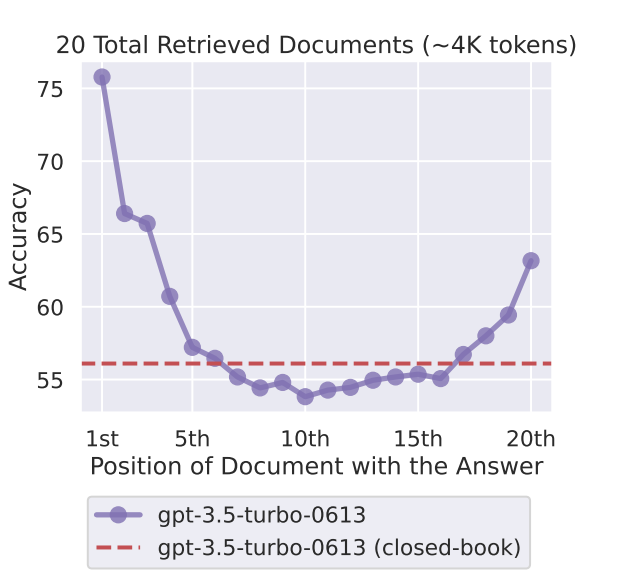
\includegraphics[width=0.5\textwidth]{assets/U-curve-diagram.png}
  \caption{La modifica della posizione delle informazioni rilevanti (in questo caso, la posizione del passaggio che risponde a una domanda in input) all'interno del contesto di input del modello linguistico produce una curva delle prestazioni a forma di U: i modelli sono più abili nell'utilizzare le informazioni rilevanti che compaiono all'inizio o alla fine del proprio contesto di input, e le prestazioni diminuiscono in modo significativo quando i modelli devono accedere e utilizzare informazioni situate nella parte centrale del proprio contesto di input. Fonte: Liu et al. \cite{liu2023lostmiddle} }
  \label{fig:u-curve}
\end{figure}

Per un sistema che costruisce il proprio contesto
unendo più frammenti recuperati, come quello di questo lavoro, questo risultato implica che l'ordine con cui i
frammenti vengono presentati al modello non è un dettaglio ininfluente quanto potrebbe sembrare a prima vista, specie
quando il numero di frammenti recuperati si avvicina al
limite superiore per cui l'effetto è stato osservato in letteratura.

\section{Sistemi che utilizzano LLM e RAG per rispondere in maniera automatica} \label{sec:sistemi-simili}

I chatbot per l'assistenza universitaria non nascono con i LLM: le prime generazioni di questi sistemi, risalenti a
ben prima della diffusione dei Transformer, si basavano su alberi di decisione scritti a mano o su classificatori
statistici, abbinati a un insieme limitato e predefinito di risposte. Erano sistemi capaci di gestire bene le
domande più frequenti, previste in fase di progettazione, ma fragili di fronte a qualunque formulazione che si
discostasse dal copione atteso. L'arrivo di LLM in grado di comprendere una domanda espressa liberamente, combinati
con il paradigma RAG per ancorare la risposta a documenti reali invece che a un insieme fisso di risposte
prestabilite, segna il passaggio a una nuova generazione di sistemi: capaci, in linea di principio, di rispondere a
qualunque domanda per cui esista un documento pertinente nella base indicizzata, senza dover prevedere a priori ogni
possibile formulazione.

L'applicazione di LLM e RAG all'assistenza universitaria non è, a questo punto, un'idea isolata. Peyton et al.
\cite{peyton2025review}, in una rassegna recente dedicata ai chatbot universitari per il supporto agli studenti,
confrontano otto implementazioni distinte e osservano come il settore non abbia ancora sfruttato appieno il
potenziale di questi sistemi rispetto ad altri ambiti applicativi, in parte per la difficoltà di reperire e curare
dataset di dominio chiuso, specifici di un singolo ateneo, su cui valutarli in modo affidabile. È un'osservazione
che motiva direttamente la scelta di questo lavoro di costruire un dataset diagnostico dedicato
(Capitolo~\ref{cap:validazione}), invece di affidarsi a benchmark generici.

Tre sistemi recenti sono particolarmente vicini, per dominio e impostazione, a quello sviluppato in questo lavoro.
Unipa-GPT \cite{siragusa2024unipagpt}, sviluppato per l'Università di Palermo, è un assistente conversazionale in
italiano rivolto a potenziali studenti che devono scegliere un corso di laurea triennale o magistrale. Gli autori
confrontano esplicitamente un approccio RAG, che recupera il contesto da un corpus raccolto dal sito web
dell'ateneo, con un approccio di fine-tuning dello stesso modello di base: un punto di riferimento diretto, su un
dominio analogo a quello di questo progetto, per la stessa alternativa architetturale discussa nella
Sezione~\ref{sec:rag}. Marcel \cite{trienes2025marcel}, sviluppato per l'Università di Marburg, si concentra invece
sulle domande più frequenti dei futuri studenti relative all'ammissione, e affianca alla ricerca sui documenti un
retriever dedicato alle FAQ: in questo modo il personale amministrativo può orientare esplicitamente le risposte
alle domande ricorrenti, invece di affidarsi interamente all'indicizzazione automatica dei documenti originali.
Vlahek \cite{vlahek2024chatbot}, infine, descrive un prototipo di chatbot RAG per il supporto agli studenti
universitari realizzato con uno strumento \emph{low-code} (Flowise AI), invece che con una pipeline sviluppata su
misura come nei due casi precedenti. Il lavoro conferma che la combinazione di LLM e RAG per questo tipo di compito
è ormai accessibile anche senza un'implementazione interamente personalizzata, benché a scapito del controllo
puntuale su ciascuno stadio della pipeline (chunking, ricerca ibrida, reranking) discusso nella
Sezione~\ref{sec:rag}, centrale nelle scelte di questo lavoro.

Il quadro non è però limitato all'ambito universitario: sistemi LLM più RAG vengono ormai distribuiti anche in
contesti industriali, e la letteratura che ne documenta la realizzazione è complementare a quella dei sistemi
accademici, perché si concentra sui problemi di ingegnerizzazione che emergono una volta messo in uso un sistema
reale, più che sulla sola qualità delle risposte misurata su un benchmark. Barnett et al.
\cite{barnett2024sevenfailures} riportano l'esperienza di tre implementazioni RAG distinte, in ambito di ricerca,
educativo e biomedico, e ne ricavano sette punti di fallimento ricorrenti. Tra questi il \emph{missing content}, in
cui il documento necessario a rispondere non è presente nella base indicizzata, e il \emph{missed top-ranked
document}, in cui il documento pertinente esiste nell'indice ma non emerge tra i candidati restituiti dal recupero.
Gli autori osservano inoltre che la robustezza di un sistema RAG si costruisce iterativamente con l'uso reale e non
può essere interamente garantita in fase di progettazione. Bourdin et al. \cite{bourdin2025easirag} documentano un
caso concreto di questo tipo in un contesto manifatturiero: un laboratorio di test ambientali che ha realizzato un
assistente RAG per rispondere alle domande degli operatori a partire dalle procedure operative interne.

Letti insieme, i sistemi universitari descritti condividono con questo lavoro l'impostazione di fondo --- LLM più
RAG, applicato alle domande degli studenti di un singolo ateneo --- ma nessuno descrive come gestire una domanda la
cui risposta dipende dal corso di laurea dello studente, quando questa informazione non è esplicita nel testo della
domanda. Unipa-GPT e Vlahek operano su un unico corpus (rispettivamente l'intero ateneo di Palermo e un singolo
corso), dove il problema non si pone nella stessa forma; Marcel, pur limitato alle sole domande di ammissione, non
discute casi di ambiguità tra profili di studenti diversi.

È in questo spazio che si colloca il presente lavoro. Il sistema sviluppato indicizza insieme le pagine di più corsi
di laurea, le pagine generali di ateneo e i materiali didattici: la stessa domanda --- una scadenza, un requisito,
un referente --- può quindi avere risposte diverse a seconda del corso. Per questo il sistema riconosce quando una
domanda è ambigua rispetto al corso, chiede allo studente di indicarlo, e usa poi il corso noto per privilegiare i
documenti pertinenti, senza escludere quelli degli altri corsi o di ateneo. La soluzione adottata è descritta nel
Capitolo~\ref{cap:architettura} e valutata nel Capitolo~\ref{cap:validazione}.

